%-------------------------------------------------------------------------
% ds-info-S1-tests.tex
%-------------------------------------------------------------------------

%-------------------------------------------------------------------------
\documentclass[11pt,a4paper]{article}
%-------------------------------------------------------------------------

%-------------------------------------------------------------------------
\input{ds-info-S1-preambule.tex}
%-------------------------------------------------------------------------

%-------------------------------------------------------------------------
\begin{document}
%-------------------------------------------------------------------------
%\noindent\framebox[\textwidth]{}
\entete

\autoevaluation


$$\mbox{\textbf{\large Graphes de fonctions}}$$


%-------------------------------------------------------------------------
%\newpage
\paragraph{Questions :}
%-------------------------------------------------------------------------
Ecrire une alternative multiple qui permette
de déterminer $y = f(x)$ pour une fonction $f$ définie par son graphe
sur $[-5;5]$ et $\forall x < -5, f(x) = f(-5)$
et $\forall x > 5, f(x) = f(5)$.

\noindent\begin{minipage}[t]{7.75cm}
\begin{enumerate}\setcounter{enumi}{0}

\item \begin{minipage}{6.75cm}
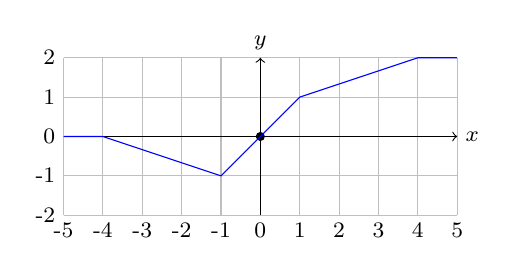
\begin{tikzpicture}[scale=0.5]\footnotesize
\draw[color=lightgray](-5,-2) grid[xstep=1,ystep=1] (5,2);
\foreach \x in {-5,-4,...,5} \draw(\x,-2) node[below]{\x};
\foreach \y in {-2,-1,...,2} \draw(-5,\y) node[left]{\y};
\filldraw(0,0) circle (0.1);
\draw[->] (-5,0) -- (5,0);
\draw (5,0) node[right]{$x$} ;
\draw[->] (0,-2) -- (0,2);
\draw (0,2) node[above]{$y$};
\draw[color=blue] (-5,0) -- (-4,0) -- (-1,-1) -- (1,1) -- (4,2) -- (5,2);
\end{tikzpicture}
\end{minipage}

\item \begin{minipage}{6.75cm}
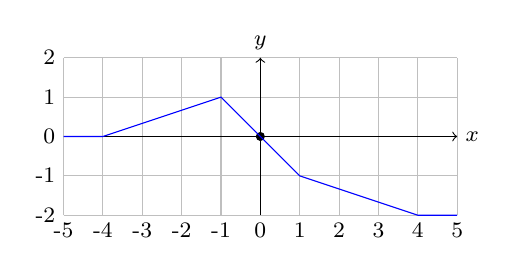
\begin{tikzpicture}[scale=0.5]\footnotesize
\draw[color=lightgray](-5,-2) grid[xstep=1,ystep=1] (5,2);
\foreach \x in {-5,-4,...,5} \draw(\x,-2) node[below]{\x};
\foreach \y in {-2,-1,...,2} \draw(-5,\y) node[left]{\y};
\filldraw(0,0) circle (0.1);
\draw[->] (-5,0) -- (5,0); 
\draw (5,0) node[right]{$x$} ;
\draw[->] (0,-2) -- (0,2);
\draw (0,2) node[above]{$y$};
\draw[color=blue] (-5,0) -- (-4,0) -- (-1,1) -- (1,-1) -- (4,-2) -- (5,-2);
\end{tikzpicture}
\end{minipage}

\item \begin{minipage}{6.75cm}
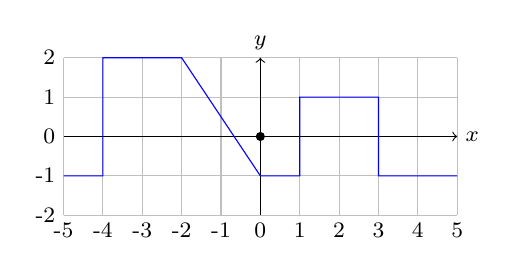
\begin{tikzpicture}[scale=0.5]\footnotesize
\draw[color=lightgray](-5,-2) grid[xstep=1,ystep=1] (5,2);
\foreach \x in {-5,-4,...,5} \draw(\x,-2) node[below]{\x};
\foreach \y in {-2,-1,...,2} \draw(-5,\y) node[left]{\y};
\filldraw(0,0) circle (0.1);
\draw[->] (-5,0) -- (5,0);
\draw (5,0) node[right]{$x$} ;
\draw[->] (0,-2) -- (0,2);
\draw (0,2) node[above]{$y$};
\draw[color=blue] (-5,-1) -- (-4,-1) -- (-4,2) -- (-2,2) -- (0,-1) -- (1,-1) -- (1,1) -- (3,1) -- (3,-1) -- (5,-1);
\end{tikzpicture}
\end{minipage}

\item \begin{minipage}{6.75cm}
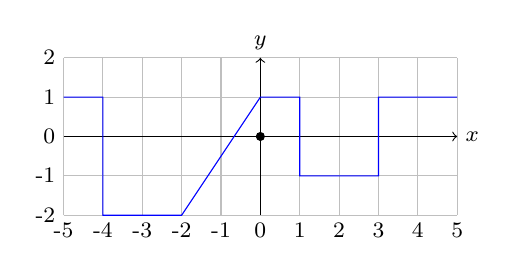
\begin{tikzpicture}[scale=0.5]\footnotesize
\draw[color=lightgray](-5,-2) grid[xstep=1,ystep=1] (5,2);
\foreach \x in {-5,-4,...,5} \draw(\x,-2) node[below]{\x};
\foreach \y in {-2,-1,...,2} \draw(-5,\y) node[left]{\y};
\filldraw(0,0) circle (0.1);
\draw[->] (-5,0) -- (5,0); 
\draw (5,0) node[right]{$x$} ;
\draw[->] (0,-2) -- (0,2);
\draw (0,2) node[above]{$y$};
\draw[color=blue] (-5,1) -- (-4,1) -- (-4,-2) -- (-2,-2) -- (0,1) -- (1,1) -- (1,-1) -- (3,-1) -- (3,1) -- (5,1);
\end{tikzpicture}
\end{minipage}

\item \begin{minipage}{6.75cm}
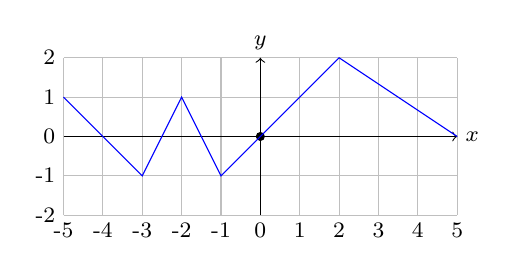
\begin{tikzpicture}[scale=0.5]\footnotesize
\draw[color=lightgray](-5,-2) grid[xstep=1,ystep=1] (5,2);
\foreach \x in {-5,-4,...,5} \draw(\x,-2) node[below]{\x};
\foreach \y in {-2,-1,...,2} \draw(-5,\y) node[left]{\y};
\filldraw(0,0) circle (0.1);
\draw[->] (-5,0) -- (5,0);
\draw (5,0) node[right]{$x$} ;
\draw[->] (0,-2) -- (0,2);
\draw (0,2) node[above]{$y$};
\draw[color=blue] (-5,1) -- (-3,-1) -- (-2,1) -- (-1,-1) -- (2,2) -- (5,0);
\end{tikzpicture}
\end{minipage}

\end{enumerate}
\end{minipage}
\hfill
\begin{minipage}[t]{7.75cm}
\begin{enumerate}\setcounter{enumi}{5}

\item \begin{minipage}{6.75cm}
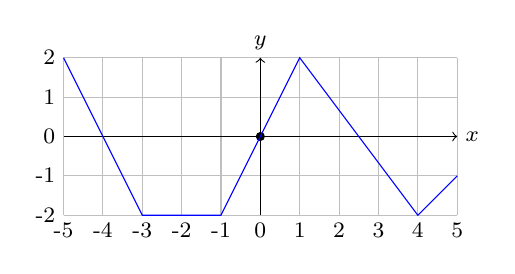
\begin{tikzpicture}[scale=0.5]\footnotesize
\draw[color=lightgray](-5,-2) grid[xstep=1,ystep=1] (5,2);
\foreach \x in {-5,-4,...,5} \draw(\x,-2) node[below]{\x};
\foreach \y in {-2,-1,...,2} \draw(-5,\y) node[left]{\y};
\filldraw(0,0) circle (0.1);
\draw[->] (-5,0) -- (5,0); 
\draw (5,0) node[right]{$x$} ;
\draw[->] (0,-2) -- (0,2);
\draw (0,2) node[above]{$y$};
\draw[color=blue] (-5,2) -- (-3,-2) -- (-1,-2) -- (1,2) -- (4,-2) -- (5,-1);
\end{tikzpicture}
\end{minipage}

\item \begin{minipage}{6.75cm}
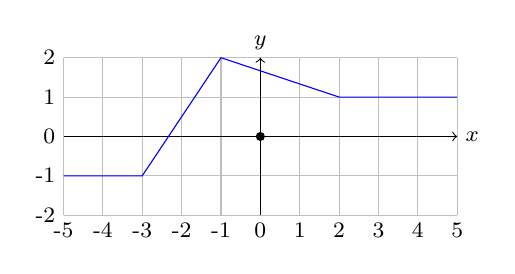
\begin{tikzpicture}[scale=0.5]\footnotesize
\draw[color=lightgray](-5,-2) grid[xstep=1,ystep=1] (5,2);
\foreach \x in {-5,-4,...,5} \draw(\x,-2) node[below]{\x};
\foreach \y in {-2,-1,...,2} \draw(-5,\y) node[left]{\y};
\filldraw(0,0) circle (0.1);
\draw[->] (-5,0) -- (5,0);
\draw (5,0) node[right]{$x$} ;
\draw[->] (0,-2) -- (0,2);
\draw (0,2) node[above]{$y$};
\draw[color=blue] (-5,-1) -- (-3,-1) -- (-1,2) -- (2,1) -- (4,1) -- (5,1);
\end{tikzpicture}
\end{minipage}

\item \begin{minipage}{6.75cm}
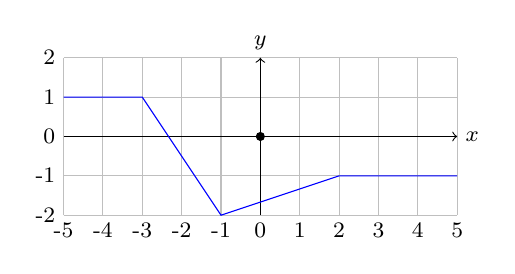
\begin{tikzpicture}[scale=0.5]\footnotesize
\draw[color=lightgray](-5,-2) grid[xstep=1,ystep=1] (5,2);
\foreach \x in {-5,-4,...,5} \draw(\x,-2) node[below]{\x};
\foreach \y in {-2,-1,...,2} \draw(-5,\y) node[left]{\y};
\filldraw(0,0) circle (0.1);
\draw[->] (-5,0) -- (5,0); 
\draw (5,0) node[right]{$x$} ;
\draw[->] (0,-2) -- (0,2);
\draw (0,2) node[above]{$y$};
\draw[color=blue] (-5,1) -- (-3,1) -- (-1,-2) -- (2,-1) -- (4,-1) -- (5,-1);
\end{tikzpicture}
\end{minipage}

\item \begin{minipage}{6.75cm}
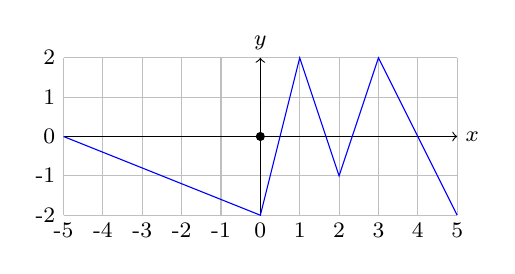
\begin{tikzpicture}[scale=0.5]\footnotesize
\draw[color=lightgray](-5,-2) grid[xstep=1,ystep=1] (5,2);
\foreach \x in {-5,-4,...,5} \draw(\x,-2) node[below]{\x};
\foreach \y in {-2,-1,...,2} \draw(-5,\y) node[left]{\y};
\filldraw(0,0) circle (0.1);
\draw[->] (-5,0) -- (5,0);
\draw (5,0) node[right]{$x$} ;
\draw[->] (0,-2) -- (0,2);
\draw (0,2) node[above]{$y$};
\draw[color=blue] (-5,0) -- (0,-2) -- (1,2) -- (2,-1) -- (3,2) -- (5,-2);
\end{tikzpicture}
\end{minipage}

\item \begin{minipage}{6.75cm}
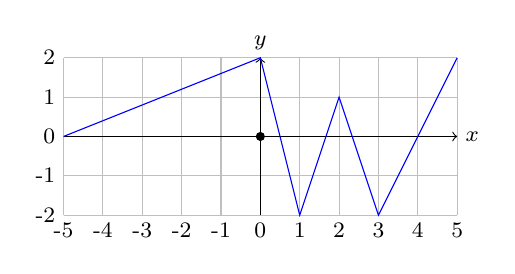
\begin{tikzpicture}[scale=0.5]\footnotesize
\draw[color=lightgray](-5,-2) grid[xstep=1,ystep=1] (5,2);
\foreach \x in {-5,-4,...,5} \draw(\x,-2) node[below]{\x};
\foreach \y in {-2,-1,...,2} \draw(-5,\y) node[left]{\y};
\filldraw(0,0) circle (0.1);
\draw[->] (-5,0) -- (5,0); 
\draw (5,0) node[right]{$x$} ;
\draw[->] (0,-2) -- (0,2);
\draw (0,2) node[above]{$y$};
\draw[color=blue] (-5,0) -- (0,2) -- (1,-2) -- (2,1) -- (3,-2) -- (5,2);
\end{tikzpicture}
\end{minipage}

\end{enumerate}
\end{minipage}

\noindent\begin{minipage}{7.75cm}
\begin{enumerate}\setcounter{enumi}{10}
\item \begin{minipage}{6.75cm}
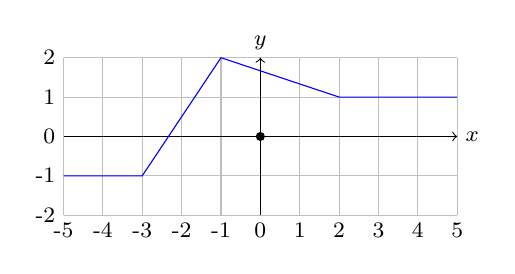
\begin{tikzpicture}[scale=0.5]\footnotesize
\draw[color=lightgray](-5,-2) grid[xstep=1,ystep=1] (5,2);
\foreach \x in {-5,-4,...,5} \draw(\x,-2) node[below]{\x};
\foreach \y in {-2,-1,...,2} \draw(-5,\y) node[left]{\y};
\filldraw(0,0) circle (0.1);
\draw[->] (-5,0) -- (5,0);
\draw (5,0) node[right]{$x$} ;
\draw[->] (0,-2) -- (0,2);
\draw (0,2) node[above]{$y$};
\draw[color=blue] (-5,-1) -- (-3,-1) -- (-1,2) -- (2,1) -- (4,1) -- (5,1);
\end{tikzpicture}
\end{minipage}

\item \begin{minipage}{6.75cm}
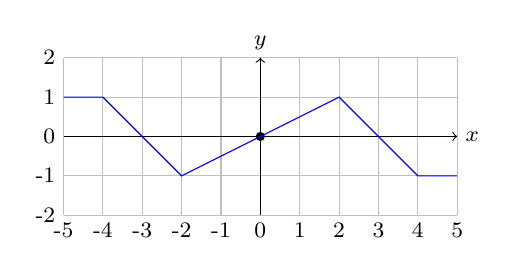
\begin{tikzpicture}[scale=0.5]\footnotesize
\draw[color=lightgray](-5,-2) grid[xstep=1,ystep=1] (5,2);
\foreach \x in {-5,-4,...,5} \draw(\x,-2) node[below]{\x};
\foreach \y in {-2,-1,...,2} \draw(-5,\y) node[left]{\y};
\filldraw(0,0) circle (0.1);
\draw[->] (-5,0) -- (5,0);
\draw (5,0) node[right]{$x$} ;
\draw[->] (0,-2) -- (0,2);
\draw (0,2) node[above]{$y$};
\draw[color=blue] (-5,1) -- (-4,1) -- (-2,-1) -- (2,1) -- (4,-1) -- (5,-1);
\end{tikzpicture}
\end{minipage}

\item \begin{minipage}{6.75cm}
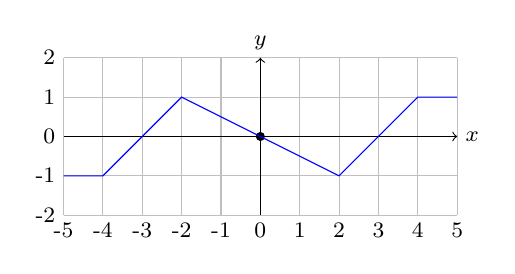
\begin{tikzpicture}[scale=0.5]\footnotesize
\draw[color=lightgray](-5,-2) grid[xstep=1,ystep=1] (5,2);
\foreach \x in {-5,-4,...,5} \draw(\x,-2) node[below]{\x};
\foreach \y in {-2,-1,...,2} \draw(-5,\y) node[left]{\y};
\filldraw(0,0) circle (0.1);
\draw[->] (-5,0) -- (5,0); 
\draw (5,0) node[right]{$x$} ;
\draw[->] (0,-2) -- (0,2);
\draw (0,2) node[above]{$y$};
\draw[color=blue] (-5,-1) -- (-4,-1) -- (-2,1) -- (2,-1) -- (4,1) -- (5,1);
\end{tikzpicture}
\end{minipage}

\item \begin{minipage}{6.75cm}
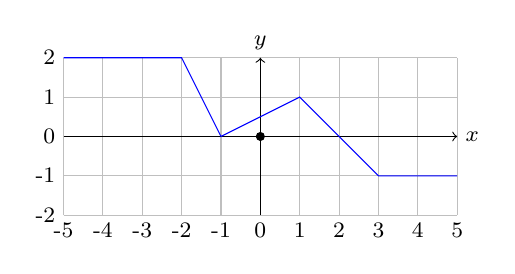
\begin{tikzpicture}[scale=0.5]\footnotesize
\draw[color=lightgray](-5,-2) grid[xstep=1,ystep=1] (5,2);
\foreach \x in {-5,-4,...,5} \draw(\x,-2) node[below]{\x};
\foreach \y in {-2,-1,...,2} \draw(-5,\y) node[left]{\y};
\filldraw(0,0) circle (0.1);
\draw[->] (-5,0) -- (5,0);
\draw (5,0) node[right]{$x$} ;
\draw[->] (0,-2) -- (0,2);
\draw (0,2) node[above]{$y$};
\draw[color=blue] (-5,2) -- (-2,2) -- (-1,0) -- (1,1) -- (3,-1) -- (5,-1);
\end{tikzpicture}
\end{minipage}

\item \begin{minipage}{6.75cm}
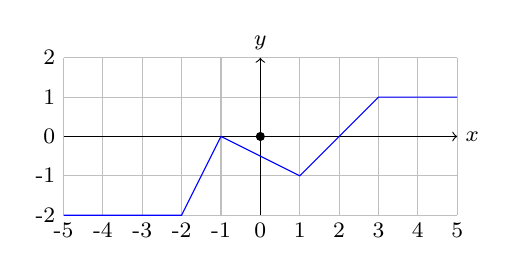
\begin{tikzpicture}[scale=0.5]\footnotesize
\draw[color=lightgray](-5,-2) grid[xstep=1,ystep=1] (5,2);
\foreach \x in {-5,-4,...,5} \draw(\x,-2) node[below]{\x};
\foreach \y in {-2,-1,...,2} \draw(-5,\y) node[left]{\y};
\filldraw(0,0) circle (0.1);
\draw[->] (-5,0) -- (5,0); 
\draw (5,0) node[right]{$x$} ;
\draw[->] (0,-2) -- (0,2);
\draw (0,2) node[above]{$y$};
\draw[color=blue] (-5,-2) -- (-2,-2) -- (-1,0) -- (1,-1) -- (3,1) -- (5,1);
\end{tikzpicture}
\end{minipage}

\item \begin{minipage}{6.75cm}
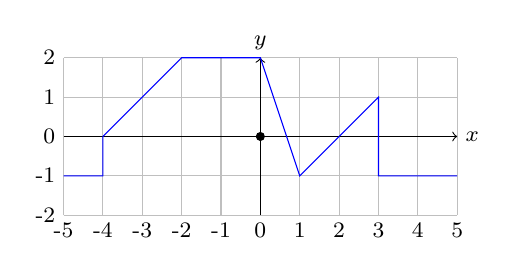
\begin{tikzpicture}[scale=0.5]\footnotesize
\draw[color=lightgray](-5,-2) grid[xstep=1,ystep=1] (5,2);
\foreach \x in {-5,-4,...,5} \draw(\x,-2) node[below]{\x};
\foreach \y in {-2,-1,...,2} \draw(-5,\y) node[left]{\y};
\filldraw(0,0) circle (0.1);
\draw[->] (-5,0) -- (5,0);
\draw (5,0) node[right]{$x$} ;
\draw[->] (0,-2) -- (0,2);
\draw (0,2) node[above]{$y$};
\draw[color=blue] (-5,-1) -- (-4,-1) -- (-4,0) -- (-2,2) -- (0,2) -- (1,-1) -- (1,-1) -- (3,1) -- (3,-1) -- (5,-1);
\end{tikzpicture}
\end{minipage}

\item \begin{minipage}{6.75cm}
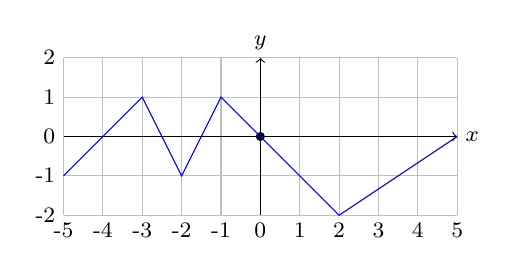
\begin{tikzpicture}[scale=0.5]\footnotesize
\draw[color=lightgray](-5,-2) grid[xstep=1,ystep=1] (5,2);
\foreach \x in {-5,-4,...,5} \draw(\x,-2) node[below]{\x};
\foreach \y in {-2,-1,...,2} \draw(-5,\y) node[left]{\y};
\filldraw(0,0) circle (0.1);
\draw[->] (-5,0) -- (5,0); 
\draw (5,0) node[right]{$x$} ;
\draw[->] (0,-2) -- (0,2);
\draw (0,2) node[above]{$y$};
\draw[color=blue] (-5,-1) -- (-3,1) -- (-2,-1) -- (-1,1) -- (2,-2) -- (5,0);
\end{tikzpicture}
\end{minipage}

\end{enumerate}
\end{minipage}
\hfill
\begin{minipage}{7.75cm}
\begin{enumerate}\setcounter{enumi}{17}

\item \begin{minipage}{6.75cm}
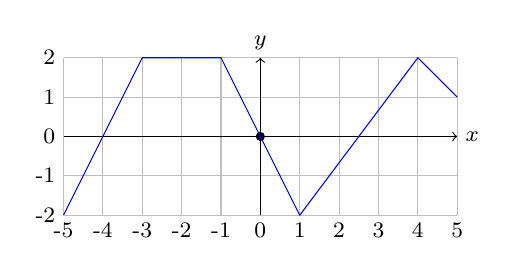
\begin{tikzpicture}[scale=0.5]\footnotesize
\draw[color=lightgray](-5,-2) grid[xstep=1,ystep=1] (5,2);
\foreach \x in {-5,-4,...,5} \draw(\x,-2) node[below]{\x};
\foreach \y in {-2,-1,...,2} \draw(-5,\y) node[left]{\y};
\filldraw(0,0) circle (0.1);
\draw[->] (-5,0) -- (5,0);
\draw (5,0) node[right]{$x$} ;
\draw[->] (0,-2) -- (0,2);
\draw (0,2) node[above]{$y$};
\draw[color=blue] (-5,-2) -- (-3,2) -- (-1,2) -- (1,-2) -- (4,2) -- (5,1);
\end{tikzpicture}
\end{minipage}

\item \begin{minipage}{6.75cm}
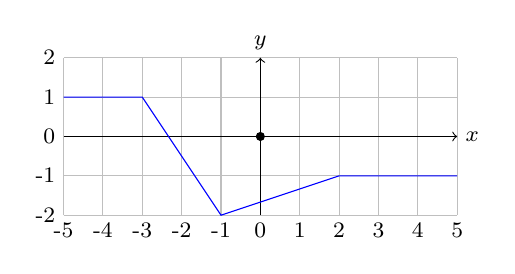
\begin{tikzpicture}[scale=0.5]\footnotesize
\draw[color=lightgray](-5,-2) grid[xstep=1,ystep=1] (5,2);
\foreach \x in {-5,-4,...,5} \draw(\x,-2) node[below]{\x};
\foreach \y in {-2,-1,...,2} \draw(-5,\y) node[left]{\y};
\filldraw(0,0) circle (0.1);
\draw[->] (-5,0) -- (5,0); 
\draw (5,0) node[right]{$x$} ;
\draw[->] (0,-2) -- (0,2);
\draw (0,2) node[above]{$y$};
\draw[color=blue] (-5,1) -- (-3,1) -- (-1,-2) -- (2,-1) -- (4,-1) -- (5,-1);
\end{tikzpicture}
\end{minipage}

\item \begin{minipage}{6.75cm}
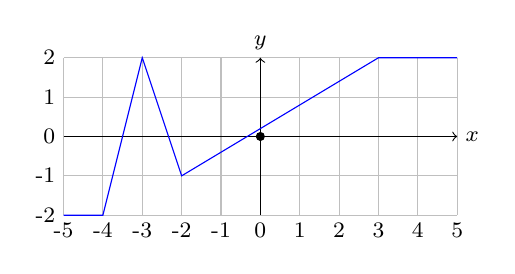
\begin{tikzpicture}[scale=0.5]\footnotesize
\draw[color=lightgray](-5,-2) grid[xstep=1,ystep=1] (5,2);
\foreach \x in {-5,-4,...,5} \draw(\x,-2) node[below]{\x};
\foreach \y in {-2,-1,...,2} \draw(-5,\y) node[left]{\y};
\filldraw(0,0) circle (0.1);
\draw[->] (-5,0) -- (5,0);
\draw (5,0) node[right]{$x$} ;
\draw[->] (0,-2) -- (0,2);
\draw (0,2) node[above]{$y$};
\draw[color=blue] (-5,-2) -- (-4,-2) -- (-3,2) -- (-2,-1) -- (3,2) -- (5,2);
\end{tikzpicture}
\end{minipage}

\item \begin{minipage}{6.75cm}
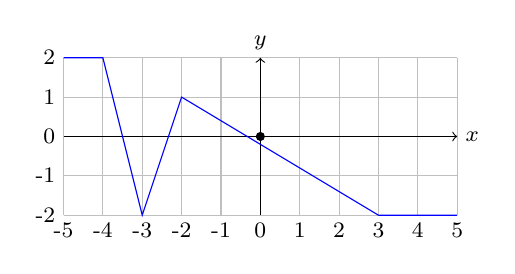
\begin{tikzpicture}[scale=0.5]\footnotesize
\draw[color=lightgray](-5,-2) grid[xstep=1,ystep=1] (5,2);
\foreach \x in {-5,-4,...,5} \draw(\x,-2) node[below]{\x};
\foreach \y in {-2,-1,...,2} \draw(-5,\y) node[left]{\y};
\filldraw(0,0) circle (0.1);
\draw[->] (-5,0) -- (5,0); 
\draw (5,0) node[right]{$x$} ;
\draw[->] (0,-2) -- (0,2);
\draw (0,2) node[above]{$y$};
\draw[color=blue] (-5,2) -- (-4,2) -- (-3,-2) -- (-2,1) -- (3,-2) -- (5,-2);
\end{tikzpicture}
\end{minipage}

\item \begin{minipage}{6.75cm}
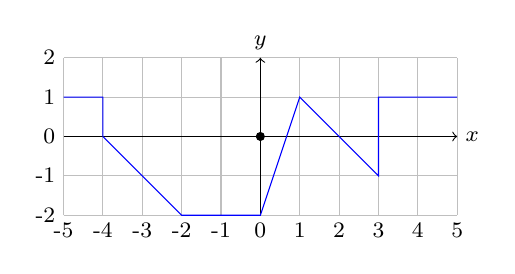
\begin{tikzpicture}[scale=0.5]\footnotesize
\draw[color=lightgray](-5,-2) grid[xstep=1,ystep=1] (5,2);
\foreach \x in {-5,-4,...,5} \draw(\x,-2) node[below]{\x};
\foreach \y in {-2,-1,...,2} \draw(-5,\y) node[left]{\y};
\filldraw(0,0) circle (0.1);
\draw[->] (-5,0) -- (5,0); 
\draw (5,0) node[right]{$x$} ;
\draw[->] (0,-2) -- (0,2);
\draw (0,2) node[above]{$y$};
\draw[color=blue] (-5,1) -- (-4,1) -- (-4,0) -- (-2,-2) -- (0,-2) -- (1,1) -- (1,1) -- (3,-1) -- (3,1) -- (5,1);
\end{tikzpicture}
\end{minipage}

\item \begin{minipage}{6.75cm}
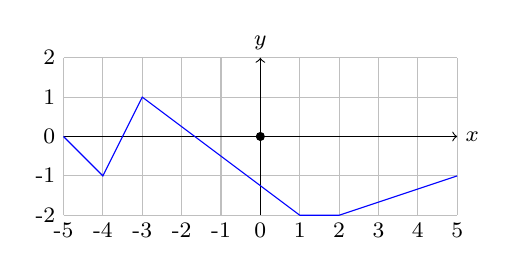
\begin{tikzpicture}[scale=0.5]\footnotesize
\draw[color=lightgray](-5,-2) grid[xstep=1,ystep=1] (5,2);
\foreach \x in {-5,-4,...,5} \draw(\x,-2) node[below]{\x};
\foreach \y in {-2,-1,...,2} \draw(-5,\y) node[left]{\y};
\filldraw(0,0) circle (0.1);
\draw[->] (-5,0) -- (5,0); 
\draw (5,0) node[right]{$x$} ;
\draw[->] (0,-2) -- (0,2);
\draw (0,2) node[above]{$y$};
\draw[color=blue] (-5,0) -- (-4,-1) -- (-3,1) -- (1,-2) -- (2,-2) -- (5,-1);
\end{tikzpicture}
\end{minipage}

\item \begin{minipage}{6.75cm}
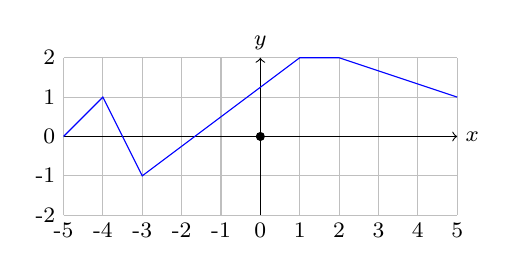
\begin{tikzpicture}[scale=0.5]\footnotesize
\draw[color=lightgray](-5,-2) grid[xstep=1,ystep=1] (5,2);
\foreach \x in {-5,-4,...,5} \draw(\x,-2) node[below]{\x};
\foreach \y in {-2,-1,...,2} \draw(-5,\y) node[left]{\y};
\filldraw(0,0) circle (0.1);
\draw[->] (-5,0) -- (5,0);
\draw (5,0) node[right]{$x$} ;
\draw[->] (0,-2) -- (0,2);
\draw (0,2) node[above]{$y$};
\draw[color=blue] (-5,0) -- (-4,1) -- (-3,-1) -- (1,2) -- (2,2) -- (5,1);
\end{tikzpicture}
\end{minipage}

\end{enumerate}
\end{minipage}

%-------------------------------------------------------------------------
\newpage
\paragraph{Réponse :}\mbox{}\ 

\noindent\framebox[\textwidth]{$\rule{0cm}{0.96\textheight}$}

%-------------------------------------------------------------------------
\end{document}
%-------------------------------------------------------------------------

